\section{Agent-Based Simulations}
\label{sec:section4}  
\subsection{Convergence and Dynamics}
Given the lack of accessible SBDA user data, I developed on agent-based simulation environment to explore the evolution of both behavioural and market-level dynamics under the above theoretical foundations. Agent-based modelling (ABM) aims to explore ``how macro phenomena emerges from micro level behaviour among a heterogeneous set of interacting agents'' \citep{janssen2005agent}. In essence, this methodology aims to study complex dynamical processes through computational simulations, as opposed to determining closed-form solutions for these through heavily simplified assumptions, which can sometimes result in large differences between predicted and real-life trajectories for complex systems (such as markets).
When applied in combination with a micro-founded theoretical model, ABM can provide powerful insights by aiding in the identification of equilibrium states, which can be computationally expensive to approximate (and in some cases even non-existent).

\begin{figure}[ht]
    \centering
    \caption{Agent-Based Simulation Convergence}
    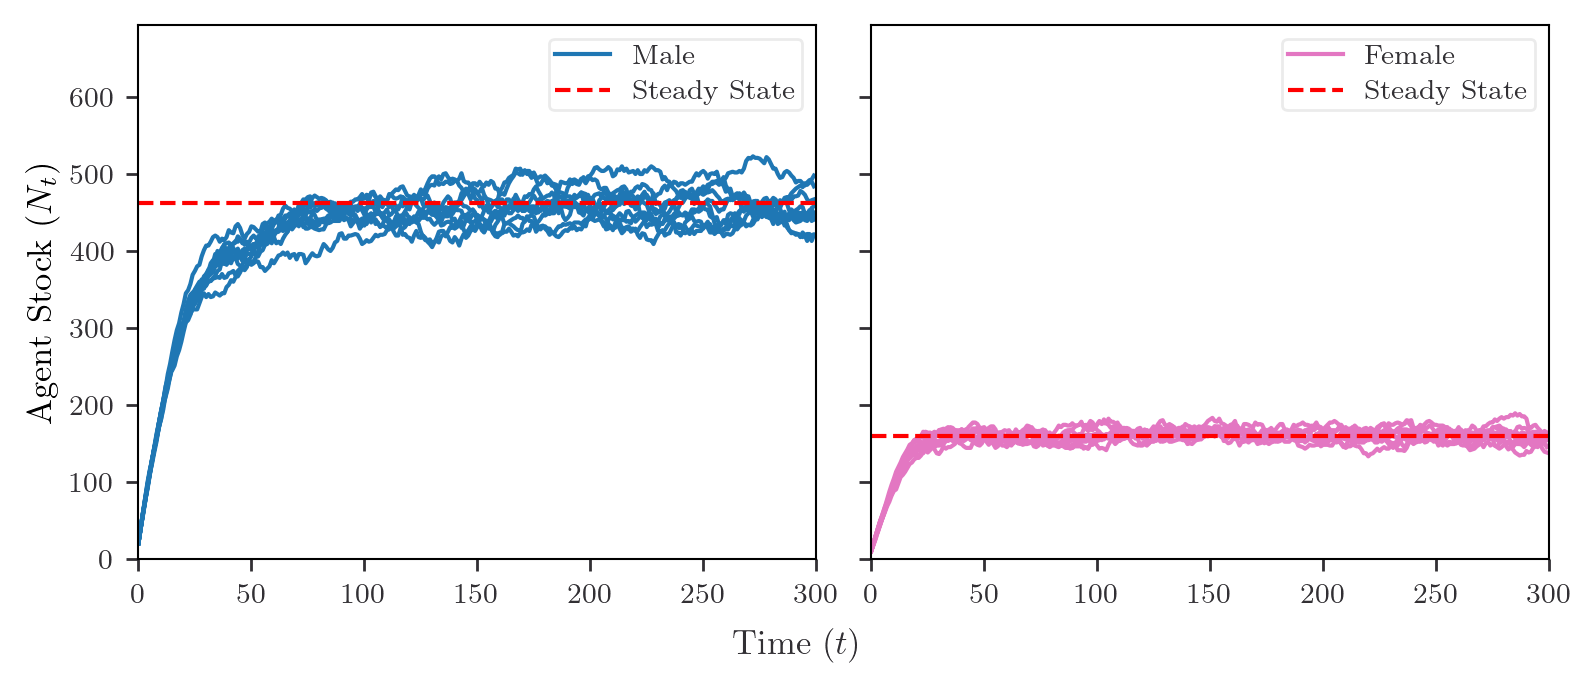
\includegraphics{abm-conv-imbalanced.png}
    \label{fig:abm-conv} 
\end{figure}

To start, I explored the convergence and stability of the SBDA market using various arbitrary exogenous settings. In particular, \autoref{fig:abm-conv} shows the simulated evolution of (sex-specific) agent masses over 300 time periods, with a 2:1 ratio between male and female arrival flows. This simulation was conducted under PREE conditions; that is, with agents playing according to the optimal policies for some fixed steady state even when this is not equal to the current platform state. As evident from these results, the computational procedures in \autoref{sec:section3.1} are able to correctly predict the steady state market masses; furthermore, the ABM simulations show that the long side of the market (males) takes considerably longer to converge onto its steady-state level. One technical point worth noting is that, due to the inability of computational simulations in handling non-discrete structures, the above simulations depict \textit{agent stocks} as opposed to \textit{agent masses}, as per our continuum model. Thus, because agent departures and pairings follow random processes, the above equilibrium acts as a \textit{stochastic steady state}, with convergence occurring in the stationary sense rather than in typical deterministic fashion. Nevertheless, I examine the limiting case of these dynamics, with \autoref{fig:abm-conv-ssize} depicting how, by the law of large numbers, stationary deviations around the steady state equilibrium level become negligible as the agent stocks tend to infinity. 

\begin{figure}[ht] 
    \centering
    \caption{Agent-Based Simulation Convergence with Varying Sample Sizes}
    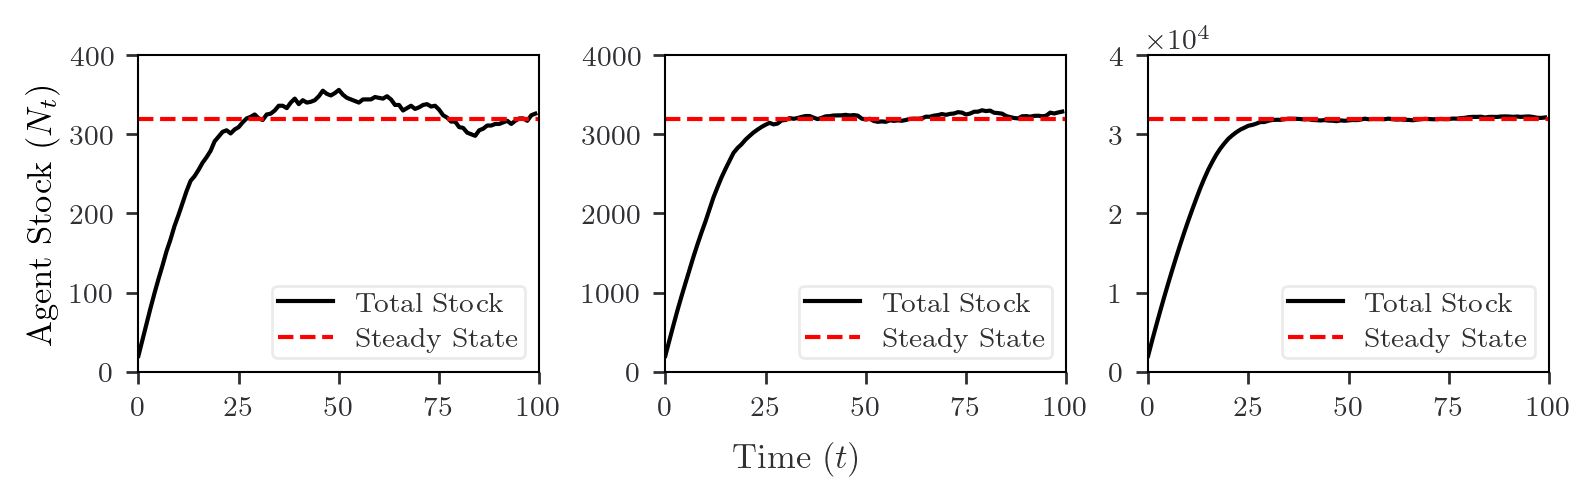
\includegraphics{abm-conv-ssize.png}
    \label{fig:abm-conv-ssize}
\end{figure} 


\begin{figure}[ht] 
    \centering
    \caption{Agent-Based Simulation Best Response Dynamics}
    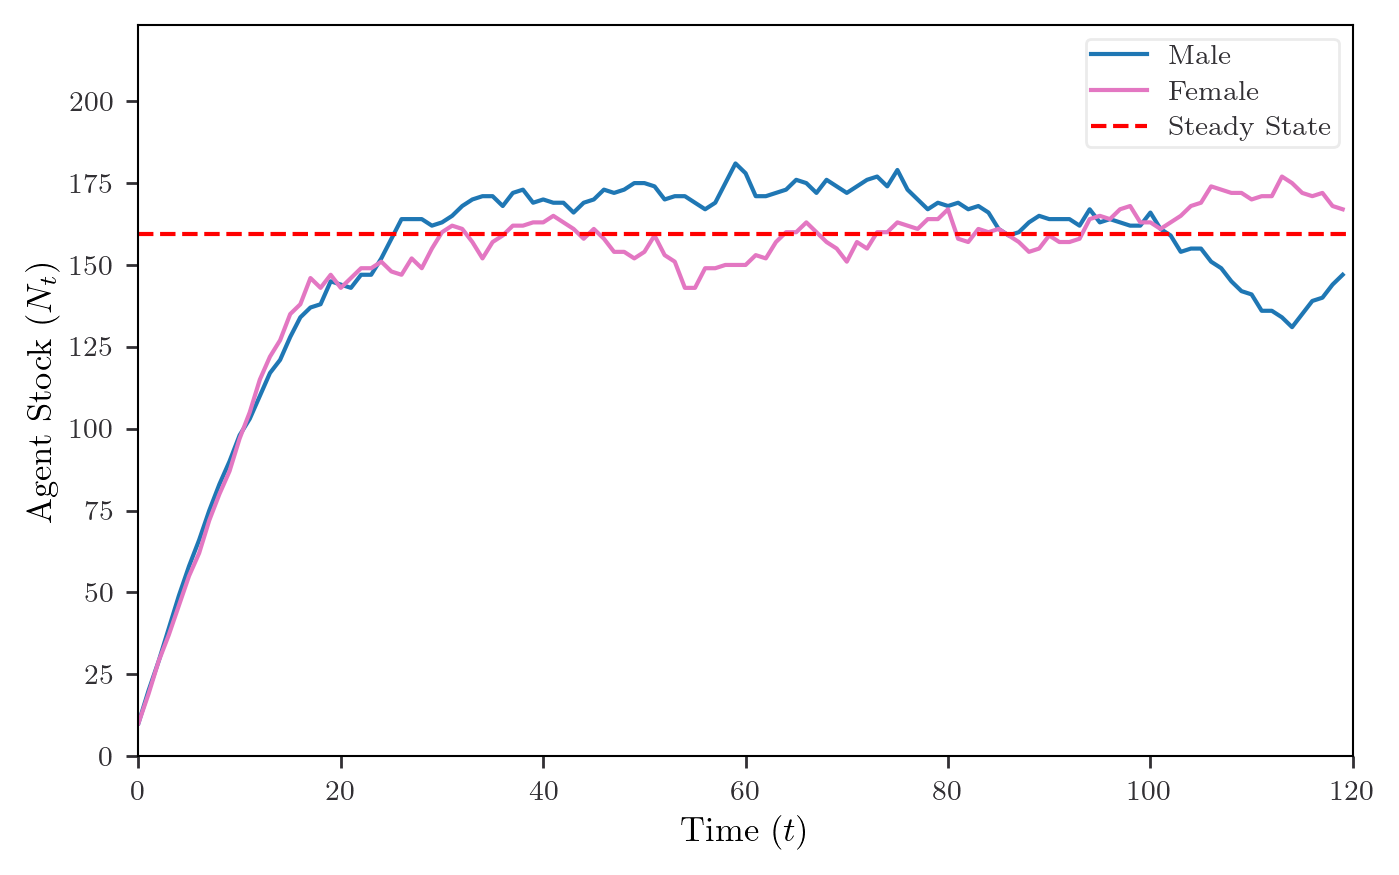
\includegraphics{abm-br-balanced.png}
    \label{fig:abm-br-balanced}
\end{figure} 
\subsection{Social Efficiency}


